\documentclass[a4paper,UTF8]{article}
\usepackage{ctex}
\usepackage[margin=1.25in]{geometry}
\usepackage{color}
\usepackage{graphicx}
\usepackage{amssymb}
\usepackage{amsmath}
\usepackage{amsthm}
\usepackage{enumerate}
\usepackage{bm}
\usepackage{hyperref}
\usepackage{epsfig}
\usepackage{color}
\usepackage{tcolorbox}
\usepackage{mdframed}
\usepackage{lipsum}
\newmdtheoremenv{thm-box}{myThm}
\newmdtheoremenv{prop-box}{Proposition}
\newmdtheoremenv{def-box}{定义}

\setlength{\evensidemargin}{.25in}
\setlength{\textwidth}{6in}
\setlength{\topmargin}{-0.5in}
\setlength{\topmargin}{-0.5in}
% \setlength{\textheight}{9.5in}
%%%%%%%%%%%%%%%%%%此处用于设置页眉页脚%%%%%%%%%%%%%%%%%%
\usepackage{fancyhdr}                                
\usepackage{lastpage}                                           
\usepackage{layout}                                             
\footskip = 10pt 
\pagestyle{fancy}                    % 设置页眉                 
\lhead{2018年春季}                    
\chead{机器学习导论}                                                
% \rhead{第\thepage/\pageref{LastPage}页} 
\rhead{作业一}                                                                                               
\cfoot{\thepage}                                                
\renewcommand{\headrulewidth}{1pt}  			%页眉线宽,设为0可以去页眉线
\setlength{\skip\footins}{0.5cm}    			%脚注与正文的距离           
\renewcommand{\footrulewidth}{0pt}  			%页脚线宽,设为0可以去页脚线

\makeatletter 									%设置双线页眉                                        
\def\headrule{{\if@fancyplain\let\headrulewidth\plainheadrulewidth\fi%
\hrule\@height 1.0pt \@width\headwidth\vskip1pt	%上面线为1pt粗  
\hrule\@height 0.5pt\@width\headwidth  			%下面0.5pt粗            
\vskip-2\headrulewidth\vskip-1pt}      			%两条线的距离1pt        
 \vspace{6mm}}     								%双线与下面正文之间的垂直间距              
\makeatother  

%%%%%%%%%%%%%%%%%%%%%%%%%%%%%%%%%%%%%%%%%%%%%%
\numberwithin{equation}{section}
%\usepackage[thmmarks, amsmath, thref]{ntheorem}
\newtheorem{myThm}{myThm}
\newtheorem*{myDef}{Definition}
\newtheorem*{mySol}{Solution}
\newtheorem*{myProof}{Proof}
\newcommand{\indep}{\rotatebox[origin=c]{90}{$\models$}}
\newcommand*\diff{\mathop{}\!\mathrm{d}}

\usepackage{multirow}

%--

%--
\begin{document}
\title{机器学习导论\\
作业一}
\author{151220097, 孙旭东, 248381185@qq.com}
\maketitle

\section*{学术诚信}

本课程非常重视学术诚信规范,助教老师和助教同学将不予余力地维护作业中的学术诚信规范的建立。希望所有选课学生能够对此予以重视。\footnote{参考尹一通老师\href{http://tcs.nju.edu.cn/wiki/index.php/\%E9\%9A\%8F\%E6\%9C/\%BA\%E7\%AE\%97\%E6\%B3\%95\_(Fall\_2015)}{高级算法课程}中对学术诚信的说明。}

\begin{tcolorbox}
\begin{enumerate}
  \item[(1)] 允许同学之间的相互讨论,但是{\color{red}\textbf{署你名字的工作必须由你完成}},不允许直接照搬任何已有的材料,必须独立完成作业的书写过程;
  \item[(2)] 在完成作业过程中,对他人工作(出版物、互联网资料)中文本的直接照搬(包括原文的直接复制粘贴及语句的简单修改等)都将视为剽窃,剽窃者成绩将被取消。{\color{red}\textbf{对于完成作业中有关键作用的公开资料,应予以明显引用}};
  \item[(3)] 如果发现作业之间高度相似将被判定为互相抄袭行为,{\color{red}\textbf{抄袭和被抄袭双方的成绩都将被取消}}。因此请主动防止自己的作业被他人抄袭。
\end{enumerate}
\end{tcolorbox}

\section*{作业提交注意事项}
\begin{tcolorbox}
\begin{enumerate}
  \item[(1)] 请严格参照课程网站作业提交方法一节提交作业;
  \item[(2)] 未按照要求提交作业,或提交作业格式不正确,将会被扣除部分作业分数;
  \item[(3)] 除非有特殊情况(如因病缓交),否则截止时间后不接收作业,本次作业记零分。
\end{enumerate}
\end{tcolorbox}

\newpage
\section{[25pts] Basic Probability and Statistics}
随机变量$X$的概率密度函数如下,
\begin{equation}
	f_X(x) = 
	\begin{cases}
		\frac{1}{4} & 0<x<1;\\
		\frac{3}{8} & 3<x<5;\\
		0			& \mbox{otherwise.}
	\end{cases}
\end{equation}
\begin{enumerate}[ {(}1{)}]
\item \textbf{[5pts]} 请计算随机变量$X$的累积分布函数$F_X(x)$;
\item \textbf{[10pts]} 随机变量$Y$定义为$Y = 1/X$,求随机变量$Y$对应的概率密度函数$f_Y(y)$;
\item \textbf{[10pts]} 试证明,对于非负随机变量$Z$,如下两种计算期望的公式是等价的。
\begin{equation}
	\label{eq-expect-1}
	\mathbb{E}[Z] = \int_{z=0}^{\infty}zf(z) \diff z.
\end{equation}

\begin{equation}
	\label{eq-expect-2}
	\mathbb{E}[Z] = \int_{z=0}^{\infty}\Pr[Z\geq z] \diff z.
\end{equation}

同时,请分别利用上述两种期望公式计算随机变量$X$和$Y$的期望,验证你的结论。
\end{enumerate}
\begin{mySol}
此处用于写解答(中英文均可)

\begin{enumerate}
	
\item 	
\begin{equation}
F_X(x) = 
\begin{cases}
\frac{1}{4}x & 0 \leq x<1;\\
\frac{1}{4} & 1 \leq x<3;\\
\frac{3}{8}x-\frac{7}{8} & 3 \leq x<5;\\ 
1 & x \geq 5 .
\end{cases}
\end{equation}

\item 
\begin{equation}
f_Y(y) =
\begin{cases}
\frac{3}{8y^2} & \frac{1}{5}<y<\frac{1}{3};\\
\frac{1}{4y^2} & y > 1;\\
0 & \mbox{otherwise.}
\end{cases}
\end{equation}

\item 
证明:
\begin{equation}
\begin{aligned}
\int_{z=0}^{\infty}\Pr[Z\geq z] \diff z 
&= \int_{z=0}^{\infty}(1-F_Z(z)) \diff z = \int_{z=0}^{\infty}\int_{v=z}^{\infty}f_Z(v) \diff v \diff z\\
&= \iint_{0 \leq z \leq v \leq \infty}f_Z(v) \diff v \diff z = \int_{v=0}^{\infty}f_Z(v)\int_{z=0}^{v}\diff z \diff v \\
&= \int_{v=0}^{\infty}vf_Z(v)\diff v
\end{aligned}
\end{equation}
由此可得$(1.2)$与$(1.3)$等价。\\
验证:\\
方法一:
\begin{equation}
\begin{aligned}
\mathbb{E}[X] &= \int_{x=0}^{\infty}xf(x) \diff x = \int_{0}^{1}\frac{1}{4}x\diff x + \int_{3}^{5}\frac{3}{8}x\diff x =\frac{25}{8}
\end{aligned}
\end{equation}
方法二:
\begin{equation}
\begin{aligned}
\mathbb{E}[X] &= \int_{x=0}^{\infty}\Pr[X\geq x] \diff x = \int_{0}^{1}(1-\frac{1}{4}x)\diff x 
+ \int_{1}^{3}\frac{3}{4}\diff x
+ \int_{3}^{5}(\frac{15}{8}-\frac{3}{8}x)\diff x\\
&= \frac{25}{8}
\end{aligned}
\end{equation}
方法一:
\begin{equation}
\begin{aligned}
\mathbb{E}[Y] &= \int_{y=0}^{\infty}yf(y) \diff y = \int_{\frac{1}{5}}^{\frac{1}{3}}\frac{3}{8y}\diff y + \int_{1}^{\infty}\frac{1}{4y}\diff y = \infty
\end{aligned}
\end{equation}
方法二:
\begin{equation}
F_Y(y) =
\begin{cases}
\frac{15}{8} - \frac{3}{8y} & \frac{1}{5}<y\leq\frac{1}{3};\\
\frac{3}{4} & \frac{1}{3} < y \leq 1;\\
1-\frac{1}{4y} & 1 < y;\\
0 & \mbox{otherwise.}
\end{cases}
\end{equation}

\begin{equation}
\begin{aligned}
\mathbb{E}[Y] &= \int_{y=0}^{\infty}\Pr[Y \geq y] \diff y\\ 
&= \int_{\frac{1}{5}}^{\frac{1}{3}}(\frac{3}{8y} - \frac{7}{8}) \diff y + \int_{\frac{1}{3}}^{1}\frac{1}{4}\diff y + \int_{1}^{\infty}\frac{1}{4y}\diff y =\infty
\end{aligned}
\end{equation}

\end{enumerate}

\end{mySol}

\newpage

\section{[20pts] Strong Convexity}
通过课本附录章节的学习,我们了解到凸性(convexity)对于机器学习的优化问题来说是非常良好的性质。下面,我们将引入比凸性还要好的性质——强凸性(strong convexity)。
\begin{def-box}[强凸性]
记函数$f: \mathcal{K} \rightarrow \mathbb{R}$,如果对于任意$\mathbf{x}, \mathbf{y} \in \mathcal{K}$及任意$\alpha\in[0,1]$,有以下命题成立
\begin{equation}
  \label{eq-sc-1}
  f((1-\alpha)\mathbf{x} + \alpha\mathbf{y})\leq (1-\alpha)f(\mathbf{x}) + \alpha f(\mathbf{y}) - \frac{\lambda}{2}\alpha(1-\alpha)\lVert \mathbf{x} - \mathbf{y}\rVert^2.
\end{equation}
则我们称函数$f$为关于范数$\lVert \cdot \rVert$的$\lambda$-强凸函数。
\end{def-box}

请证明,在函数$f$可微的情况下,式~\eqref{eq-sc-1}与下式~\eqref{eq-sc-2}等价,
\begin{equation}
  \label{eq-sc-2}
  f(\mathbf{y}) \geq f(\mathbf{x}) + \nabla f(\mathbf{x})^\mathrm{T}(\mathbf{y}-\mathbf{x}) + \frac{\lambda}{2}\lVert \mathbf{y} - \mathbf{x}\rVert^2.
\end{equation}
\begin{myProof}
此处用于写证明(中英文均可)

做法参考了《convex optimazition》一书。\\
先证明$(2.1) \Rightarrow (2.2)$:
\begin{equation}
\begin{aligned}
&f((1-\alpha)\mathbf{x} + \alpha\mathbf{y})\leq (1-\alpha)f(\mathbf{x}) + \alpha f(\mathbf{y}) - \frac{\lambda}{2}\alpha(1-\alpha)\lVert \mathbf{x} - \mathbf{y}\rVert^2\\
\Rightarrow &\alpha f(\mathbf{y}) \geq f(\mathbf{x}+\alpha(\mathbf{y}-\mathbf{x})) - (1-\alpha)f(\mathbf{x}) + \frac{\lambda}{2}\alpha(1-\alpha)\lVert \mathbf{x} - \mathbf{y}\rVert^2\\
\Rightarrow & f(\mathbf{y}) \geq f(\mathbf{x}) + \frac{f(\mathbf{x} + \alpha(\mathbf{y}-\mathbf{x}))-f(\mathbf{x})}{\alpha} + \frac{\lambda}{2}(1-\alpha)\lVert \mathbf{x} - \mathbf{y}\rVert^2
\end{aligned}
\end{equation}

根据导数定义
\begin{equation}
\lim\limits_{\alpha\rightarrow 0}\frac{f(\mathbf{x} + \alpha(\mathbf{y}-\mathbf{x}))-f(\mathbf{x})}{\alpha} = \nabla f(\mathbf{x})^\mathrm{T}(\mathbf{y}-\mathbf{x})	
\end{equation}
所以根据$(2.3)$和$(2.4)$可以得到$(2.1) \Rightarrow (2.2)$。\\\\
下面证明$(2.2) \Rightarrow (2.1)$:\\
因为有$f(\mathbf{y}) \geq f(\mathbf{x}) + \nabla f(\mathbf{x})^\mathrm{T}(\mathbf{y}-\mathbf{x}) + \frac{\lambda}{2}\lVert \mathbf{y} - \mathbf{x}\rVert^2$,可得:
\begin{equation}
f(\mathbf{x}) \geq f(\mathbf{z}) + \nabla f(\mathbf{z})(\mathbf{x}-\mathbf{z}) + \frac{\lambda}{2}\lVert \mathbf{x} - \mathbf{z}\rVert^2
\end{equation}

\begin{equation}
f(\mathbf{y}) \geq f(\mathbf{z}) + \nabla f(\mathbf{z})(\mathbf{y}-\mathbf{z}) + \frac{\lambda}{2}\lVert \mathbf{y} - \mathbf{z}\rVert^2
\end{equation}

其中$\mathbf{z} = (1-\alpha)\mathbf{x} + \alpha\mathbf{y}$。由$(2.5)$和$(2.6)$可以得到:
\begin{equation}
\begin{aligned}
(1-\alpha) f(\mathbf{x}) + \alpha f(\mathbf{y}) &\geq f(\mathbf{z}) + \nabla f(\mathbf{z})((1-\alpha) \mathbf{x} + \alpha \mathbf{y} - \mathbf{z}) + (1-\alpha)\frac{\lambda}{2}\lVert \mathbf{x} - \mathbf{z}\rVert^2 + \alpha\frac{\lambda}{2}\lVert \mathbf{y} - \mathbf{z}\rVert^2\\
& =f((1-\alpha)\mathbf{x}+\alpha\mathbf{y}) + (1-\alpha)\frac{\lambda}{2}\lVert \alpha(\mathbf{x} - \mathbf{y})\rVert^2 + \alpha\frac{\lambda}{2}\lVert (1-\alpha)(\mathbf{x} - \mathbf{y})\rVert^2\\
& = f((1-\alpha)\mathbf{x}+\alpha\mathbf{y}) + \frac{\lambda}{2}\alpha(1-\alpha)\lVert \mathbf{x} - \mathbf{y}\rVert^2
\end{aligned}
\end{equation}
所以可得$(2.2) \Rightarrow (2.1)$。\\\\
综上可得,在函数$f$可微的情况下,式~\eqref{eq-sc-1}与式~\eqref{eq-sc-2}等价。
\qed
\end{myProof}


\newpage
\section{[20pts] Doubly Stochastic Matrix}
随机矩阵(stochastic matrix)和双随机矩阵(doubly stochastic matrix)在机器学习中经常出现,尤其是在有限马尔科夫过程理论中,也经常出现在于运筹学、经济学、交通运输等不同领域的建模中。下面给出定义,
\begin{def-box}[随机矩阵]
设矩阵$\mathbf{X}=[x_{ij}]\in \mathbb{R}^{d\times d}$是非负矩阵,如果$\mathbf{X}$满足
\begin{equation}
\label{eq-sto-matrix}
\sum_{j=1}^d x_{ij} = 1,\quad i=1,2,\cdots,d.
\end{equation}
则称矩阵$\mathbf{X}$为随机矩阵(stochastic matrix)。如果$\mathbf{X}$还满足
\begin{equation}
\label{eq-double-sto-matrix}
\sum_{i=1}^d x_{ij} = 1,\quad j=1,2,\cdots,d.
\end{equation}
则称矩阵$\mathbf{X}$为双随机矩阵(double stochastic matrix)。
\end{def-box}
对于双随机矩阵$\mathbf{X} \in \mathbb{R}^{d\times d}$,试证明
\begin{enumerate}[ {(}1{)}]
\item \textbf{[10pts]} 矩阵$\mathbf{X}$的\href{https://en.wikipedia.org/wiki/Entropy_(information_theory)}{信息熵 (entropy)}满足$H(\mathbf{X}) \leq d\log d$.
\item \textbf{[10pts]} 矩阵$\mathbf{X}$的\href{https://en.wikipedia.org/wiki/Spectral_radius}{谱半径 (spectral radius)}$\rho(\mathbf{X})$等于1,且是$\mathbf{X}$的特征值;(提示:你可能会需要\href{https://en.wikipedia.org/wiki/Perron%E2%80%93Frobenius_theorem}{Perron–Frobenius定理},可以基于此进行证明。)
\end{enumerate}
\begin{myProof}
此处用于写证明(中英文均可)

\begin{enumerate}
\item 
因为$H(\mathbf{X})=\sum_{i=1}^{d}\sum_{j=1}^{d}x_{ij}\log \frac{1}{x_{ij}}$,所以要证明$\sum_{i=1}^{d}\sum_{j=1}^{d}x_{ij}\log \frac{1}{x_{ij}} \leq d\log d$。证明如下:\\
首先证明$\sum_{j=1}^{d}x_{ij}\log\frac{1}{x_{ij}}\leq \log d$,观察到$f(x) = x\log \frac{1}{x}\ is\ concave\ function$,所以有$\sum_{j=1}^{d}f(x_{ij}) \leq df(\frac{\sum_{j=1}^{d}x_{ij}}{d})$,又因为$(3.1)$,所以进一步有$\sum_{j=1}^{d}f(x_{ij}) \leq d\frac{1}{d}\log \frac{d}{1} = \log d$,因此可得$H(\mathbf{X})=\sum_{i=1}^{d}\sum_{j=1}^{d}x_{ij}\log \frac{1}{x_{ij}} \leq d\log d$。

\item 
参考了wiki百科中关于Perron–Frobenius定理中的Inequalities for Perron–Frobenius eigenvalue条目。\\
首先易得$1$是$\mathbf{X}$的特征值之一,对应的特征向量$\mathbf{v}$是全一向量:因为$\mathbf{X}\mathbf{v} = 1\mathbf{v}$。\\
根据Inequalities for Perron–Frobenius eigenvalue:对任意矩阵$\mathbf{A}$的特征值$\lambda$,一定有$\vert\lambda\vert\leq\max\limits_{i}\sum_{j}\vert\mathbf{A}_{ij}\vert$。又因为$\mathbf{X}$是双随机矩阵所以对于其任意特征值$\lambda$都有$\vert\lambda\vert\leq 1$,又因为$1$是$\mathbf{X}$的特征值之一,所以可得$\rho(\mathbf{X}) = \max\left\{|\lambda_1|,...,|\lambda_d|\right\} = 1$。
\end{enumerate}

\qed
\end{myProof}
\newpage
\section{[15pts] Hypothesis Testing} 
在数据集$D_1,D_2,D_3,D_4,D_5$运行了$A,B,C,D,E$五种算法,算法比较序值表如表\ref{table:ranking}所示:
\begin{table}[h]
\centering
\caption{算法比较序值表} \vspace{2mm}
\label{table:ranking}
\begin{tabular}{c|c c c c c}\hline
数据集 		& 算法$A$  	&算法$B$  	& 算法$C$ 	& 算法$D$  	&算法$E$ 	\\ \hline
$D_1$ 		& 4 		&  3  		& 5  		&  2 		& 1			\\
$D_2$ 		& 3 		&  5  		& 2  		&  1 		& 4			\\
$D_3$ 		& 4 		&  5  		& 3  		&  1 		& 2			\\ 
$D_4$ 		& 5 		&  2  		& 4  		&  1 		& 3			\\ 
$D_5$ 		& 3 		&  5  		& 2  		&  1 		& 4			\\ \hline
\end{tabular}
\end{table}

使用Friedman检验$(\alpha=0.05)$判断这些算法是否性能都相同。若不相同,进行Nemenyi后续检验$(\alpha=0.05)$,并说明性能最好的算法与哪些算法有显著差别。
\begin{mySol}
此处用于写解答(中英文均可)\\
Friedman检验:\\
由题目得$k=5$,$N=5$,根据简单计算有$r_1=3.8, r_2=4, r_3=3.2, r_4=1.2, r_5=2.8$,根据书上$(2.34)$公式可得$\tau_{\chi^2} = 9.9200$,再根据书上$(2.35)$公式可得$\tau_F=3.9365$,查书上表$2.6$可得$3.9365 > 3.007 $,所以拒绝“所有算法性能相同”这个假设。\\
Nemenyi检验:\\
查表$2.7$可得当$k=5,\alpha=0.05$时$q_\alpha=2.728$,根据书上$(2.36)$可得$CD = 2.728$。观察题目中表$1$可得$r_2-r_4 = 2.8>2.728$所以认为算法D与算法B有显著区别,其他算法之间无显著区别。
\end{mySol}

\newpage
\section{[20pts] ROC and AUC}
现在有五个测试样例,其对应的真实标记和学习器的输出值如表\ref{table:roc}所示:
\begin{table}[!h]
	\centering
	\caption{测试样例表} \vspace{2mm}\label{table:roc}
	\begin{tabular}{c|c c c c c}\hline
		样本 & $x_1$ & $x_2$ & $x_3$  & $x_4$  & $x_5$ \\
		\hline
		标记 & +  & + &  - &  +  & -\\
		\hline
		输出值 & 0.9  & 0.3 &  0.1 &  0.7  & 0.4\\
		\hline
	\end{tabular}
\end{table}
\begin{enumerate}[ {(}1{)}]
\item \textbf{[10pts]} 请画出其对应的ROC图像,并计算对应的$\mbox{AUC}$和$\ell_{rank}$的值(提示:可使用\href{https://en.wikibooks.org/wiki/LaTeX/PGF/TikZ}{TikZ包}作为\LaTeX 中的画图工具);
\item \textbf{[10pts]} 根据书上第35页中的公式(2.20)和公式(2.21),试证明\[\mbox{AUC}+\ell_{rank}=1.\]
\end{enumerate}
\begin{mySol}
此处用于写解答(中英文均可)\\
\begin{enumerate}
\item 
\begin{figure}[ht]
	\centering
	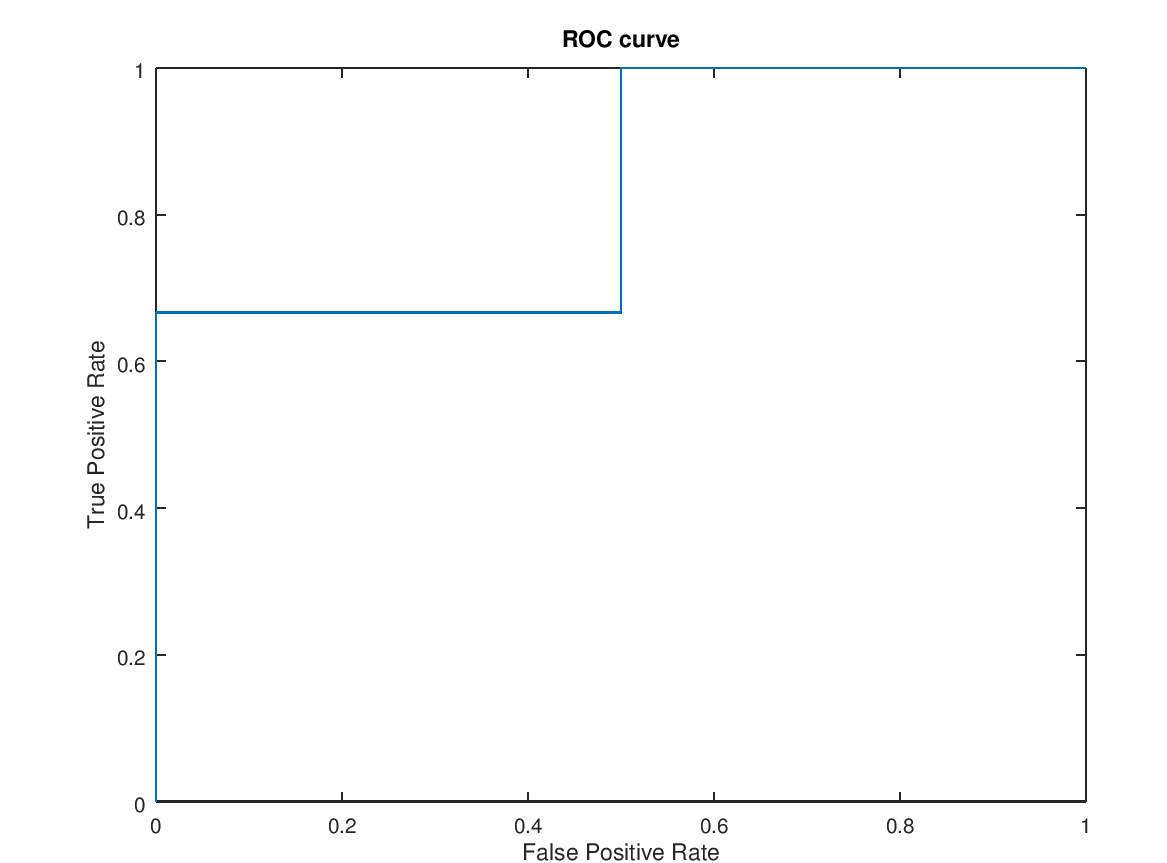
\includegraphics[scale=0.5]{roc_curve.png}
	\caption{根据表2中数据绘制的roc曲线}
	\label{fig:label}
\end{figure}
\begin{equation}
\begin{aligned}
\ell_{rank} &= \frac{1}{m^+m^-}\sum_{x^+\in D^+}\sum_{x^-\in D^-}\left(\mathbb I\left(f\left(x^+\right)<f\left(x^-\right)\right) + \frac{1}{2}\mathbb{I}\left(f\left(x^+\right)=f\left(x^-\right)\right)\right)\\
 &= \frac{1}{6}=0.1667
\end{aligned}
\end{equation}
\begin{equation}
AUC = 1-\ell_{rank} = 0.8333
\end{equation}

\item 
要证明${AUC}+\ell_{rank}=1$,即证明:
\begin{equation}
AUC = \frac{1}{m^+m^-}\sum_{x^+\in D^+}\sum_{x^-\in D^-}\left(\mathbb I\left(f\left(x^+\right)>f\left(x^-\right)\right) + \frac{1}{2}\mathbb{I}\left(f\left(x^+\right)=f\left(x^-\right)\right)\right)	
\end{equation}
根据AUC的定义可得AUC表示的是ROC曲线下方围成的面积,那么先定义一个$unit$为大小为$\frac{1}{m^+}\frac{1}{m^-}$的矩形块面积,在已知上一个样例的坐标为$(x_0, y_0)$时,如果当前样例是正样例,那么当前新坐标就是$(x_0, y_0+\frac{1}{m^+})$,并不增加面积。如果当前样例是负样例,那么当前新坐标就是$(x_0+\frac{1}{m^-}, y_0)$,会增加ROC之下的面积,增加的面积大小为k个$unit$的大小,k是输出值大于当前负样例的正样例的个数。\\
由此可得,对于任意两个一正一负的样例$s_1\in D^+$, $s_2\in D^-$,有以下三种情况:
\begin{itemize}
\item $f(s_1) > f(s_2)$,那么$s_1$和$s_2$会为AUC贡献一个$unit$的面积,因为$s_1$贡献了$\frac{1}{m^+}$的y轴长度,$s_2$贡献了$\frac{1}{m^-}$的x轴长度。
\item $f(s_1) = f(s_2)$,贡献一个三角形的面积,大小为半个$unit$大小。
\item $f(s_1) < f(s_2)$,不贡献面积。
\end{itemize}
综上所述,可得:
\begin{equation}
AUC = \frac{1}{m^+m^-}\sum_{x^+\in D^+}\sum_{x^-\in D^-}\left(\mathbb I\left(f\left(x^+\right)>f\left(x^-\right)\right) + \frac{1}{2}\mathbb{I}\left(f\left(x^+\right)=f\left(x^-\right)\right)\right)
\end{equation}
所以
\begin{equation}
AUC + \ell_{rank} = \frac{1}{m^+m^-}\sum_{x^+\in D^+}\sum_{x^-\in D^-}1 = 1
\end{equation}
\end{enumerate}
\end{mySol}

\newpage
\section{[附加题10pts] Expected Prediction Error}
对于最小二乘线性回归问题,我们假设其线性模型为:
\begin{equation}
	y=\textbf{x}^T  \bm{ \beta } + \epsilon , 
\end{equation}
其中$\epsilon$为噪声满足$\epsilon\sim N(0,\sigma^2)$。我们记训练集$\mathcal{D}$中的样本特征为$\textbf{X}\in \mathbb{R}^{p \times n}$,标记为$\textbf{Y}\in \mathbb{R}^{n}$,其中$n$为样本数,$p$为特征维度。
已知线性模型参数的估计为:
\begin{equation}
	\hat{\bm{\beta}}=(\textbf{X}\textbf{X}^T)^{-1}\textbf{X}\textbf{Y}.	
\end{equation}

对于给定的测试样本$\textbf{x}_0$,记$\mathbf{EPE}(\textbf{x}_0)$为其预测误差的期望 (Expected Predication Error),试证明,
\[
	\mathbf{EPE}(\textbf{x}_0) = \sigma^2+\mathbb{E}_{\mathcal{D}}[\textbf{x}_0^T(\textbf{X}\textbf{X}^T)^{-1}\textbf{x}_0\sigma^2].
\]

要求证明中给出详细的步骤与证明细节。(提示:$\mathbf{EPE}(\textbf{x}_0)=\mathbb{E}_{y_0|\textbf{x}_0} \mathbb{E}_{\mathcal{D}}[(y_0-\hat{y}_0)^2]$,可以参考书中第45页关于方差-偏差分解的证明过程。)

\begin{myProof}
此处用于写证明(中英文均可)
~\\
~\\
~\\
~\\
~\\

\qed
\end{myProof}




\end{document}